\documentclass[11pt,a4paper]{article}
\usepackage{amsmath, amsthm, amsfonts, amssymb}
\usepackage{color}
\usepackage{bm}	
\usepackage{float}
\usepackage{caption, subcaption}
\usepackage{times}
\usepackage{fancyhdr}           % Allows better control over headers and footers
%\usepackage{layout}            % use with \layout to see the page layout for
%debugging purposes.
\usepackage[margin=2.5cm]{geometry}  %   set the margins using the
                                %   geometry package (which is much
                                %   the easiest way of doing this).
\usepackage[pdftex]{graphicx}   %   Pictures (means you have to
                                %   produce pdf output via pdflatex)
\usepackage[small,compact]{titlesec}   % Try to reduce the white space
                                % latex loves so much
\titlelabel{\thetitle. \quad}   % Reduce space around section heads
                                % and add a full stop after the number
\pagestyle{fancy}               % Invoke fancy headers

\renewcommand{\abstractname}{\vskip -5mm}  %  Change name of Abstract
                                %  to nothing and loose some of the
                                %  excessive white space
\newcommand{\itab}[1]{\hspace{0em}\rlap{#1}}
\newcommand{\tab}[1]{\hspace{.2\textwidth}\rlap{#1}}

\begin{document}
    \begin{titlepage} \begin{center}
            \textsc{\LARGE University of Cape Town}
            \\[1.5cm] \textsc{\Large Software Engineering Stage Four} \\\smallskip
            \textsc{\Large Final Report} \\\smallskip
            \textsc{\Large CSC3003S} \\\smallskip
            \textsc{\Large \today} \\\smallskip
            \noindent\rule[0.4mm]{\textwidth}{0.1mm}
            \\[0.4cm] { \huge \bfseries Tempest Trace \\[0.4cm] }
            \noindent\rule[0.4mm]{\textwidth}{0.1mm}
            \\[1cm]
            \begin{minipage}[t]{0.4\textwidth}
                \begin{flushleft}\large \emph{Authors:}\\ Brian Mc George - MCGBRI004 \\ Jacques Heunis - HNSJAC003 \\ Timothy Gwynn - GWYTIM001
                    \\[2cm]
                \end{flushleft}
            \end{minipage} \begin{minipage}[t]{0.4\textwidth}
            \begin{flushright} \large \emph{Supervisor:} \\ Assoc. Prof.~Patrick Marais\\patrick@cs.uct.ac.za\end{flushright}
            \begin{flushright} \large \emph{Tutor:} \\ Codie Roelf\\Codie.Roelf@alumni.uct.ac.za\end{flushright}
        \end{minipage}
    \end{center}
\end{titlepage}
\newpage
\tableofcontents
\newpage

%%%  Set the headers via fancyhdr package
\lhead{Capstone Project 2015}  % Short title for running head
\chead{}
\rhead{\today}   %  Fixed running head of the date
\lfoot{}
\cfoot{\thepage}    %  add page number as centre footer.
\rfoot{}
\renewcommand{\headrulewidth}{0.0pt}   % Don't want horizontal line
                                % under header.

\begin{abstract}
The Tempest Trace project is focused around providing a two player parkour game whereby players race against each other to reach the final goal in a competitive first person runner game. Players must move over, under, around and through obstacles efficiently while avoiding enemy AI elements such as flying drones and snipers. An aspect that the game focuses on is allowing the player to choose from a variety of possible routes to gain advantage over his/her opponent; certain routes will be better in different situations so every race requires new strategies. The aesthetic is purposefully simplistic and clean to allow the player to focus on gameplay and easily identify obstacles and objects to interact with. In parkour flow and smoothness of movement are imperative and this is reflected in Tempest Trace, where the shortest path is often not the fastest and maintaining movement is often more important than achieving the highest instantaneous speed.
\end{abstract}

\section{Introduction}
\label{s:introduction}
The Tempest Trace project is a first-person running game whereby the player competes against the clock and against another player to get from the start to the end of a parkour/ free running track while trying to keep their movements smooth and free flowing. The player is tasked with traversing an obstacle course in as short a time as possible while avoiding enemies who would try to slow down or eliminate the player. In addition to this, the game will feature 2-player local multiplayer in which the players are pitted against each other to see who can complete the course the fastest. The multiplayer mode will also allow players to interact with each other, letting players try to slow their opponent down to get an edge. \\
Our development methodology included some up-front analysis of the problem in order to break it down into a more well-defined set of requirements and objectives. We then constructed an evolutionary prototype to check that the basic mechanics of the game could work and that we could implement them without too much trouble. Once the prototype was completed, we followed a roughly iterative approach, scheduling the most important features to implement or bugs to fix and then working on those for a few days before re-evaluating the state of the project and repeating the process.

\section{Requirements captured}
\subsection{Functional requirements with use case narrative}
\subsubsection{Move}
\textbf{Actor:} Player\smallskip\\
The player specifies which direction he/she wants the character to move in. The system performs collision detection to detect whether the input movement is allowed. If the movement is allowed the player's character is appropriately displaced in the system and the appropriate animation is played. The system represents this graphically for both players. The system checks whether the player has reached the end goal and if so ends the game.\smallskip\\
If the movement is not allowed the player's character will not move and no adjustments will be made to the system.

\subsubsection{Jump}
\textbf{Actor:} Player\smallskip\\
The player specifies he/she wants the character to jump. The system performs collision detection to detect whether the input movement is allowed. If the movement is allowed the player's character is appropriately displaced in the system depending on what sort of obstacle is in close proximity and in front of the player and the appropriate animation is played. If there is a low wall in front of the player, it will vault over it. If there is a taller wall the player will grab the top of the wall and pull itself up. If the wall is too tall the player will just perform the standard jump. If there is no obstacle the player will perform a standard jump. The system represents this graphically for both players and outputs appropriate sound effects. The system checks whether the player has reached the end goal and if so ends the game.\smallskip\\
If the movement is not allowed the player's character will not move and no adjustments will be made to the system.

\subsubsection{Grab ledge}
\textbf{Actor:} Player\smallskip\\
If the player jumps and hits an obstacle that does not extend above the player's head the player will grab onto the obstacle and then climb onto the obstacle. If the object extends above the player's head or is indoors (there is a ceiling above the obstacle) the movement will not be allowed.\smallskip\\
If the movement is not allowed the player's character will fall down until it encounters the floor or until the player is reset due to falling too far.

\subsubsection{Slide}
\textbf{Actor:} Player\smallskip\\
The player specifies he/she wants the character to slide. The system performs collision detection to detect whether the input movement is allowed. If the movement is allowed the player's character is appropriately displaced in the system depending on what slope is in front of the player and the appropriate animation is played. The system represents this graphically for both players and outputs appropriate sound effects. The system checks whether the player has reached the end goal and if so ends the game.\smallskip\\
If the movement is not allowed the player's character will not move and no adjustments will be made to the system.

\subsubsection{Re-spawn}
\textbf{Actor:} Player\smallskip\\
The player's character dies. The system retrieves the last re-spawn point that the player has passed. The player's character appears at the location. The system represents this graphically for both players and updates the player's character's location.  The system is updated to reflect the player's new position.\smallskip\\

\subsubsection{Use smoke grenade}
\textbf{Actor:} Player\smallskip\\
The player specifies he/she wants the character to use a smoke bomb. The system checks whether the player has smoke grenades playing. If the player has smoke grenades available the appropriate animation is displayed along with the appropriate sound effect and a new smoke cloud object is created at the player's location. Over time the smoke cloud object will shrink and eventually be removed.\smallskip\\
If the player has no smoke grenade an error sound will be played.

\subsubsection{Interact}
\textbf{Actor:} Player \smallskip \\
When the player presses the environment interaction button while near an interactable (Button or Door) the correct contextual action should occur. If the player is near a door the door should open and if the player is near a button the button should change its state to pushed and fire the script attached to it.\smallskip\\
If the player is not near an environmental object or the object has already been used (eg. door has been opened) no adjustments should be made to the system.

\subsubsection{Update drone behaviour}
\textbf{Actor:} Time\smallskip\\
Every game cycle the drone updates its behaviour. The drone checks with the system whether it has a target. If it has a target it then checks whether it is facing towards the target. If it does, it will shoot towards the target. Otherwise, it will turn to face the target. The trajectory of the bullet is offset using a function of the time the target has been tracked, distance to target and speed of target.\smallskip\\
The drone moves towards the last known location of the target if it loses sight of the target. If it cannot find the player at the last seen position it will timeout and return back to patrolling. \smallskip\\
If the drone has no target it will attempt to acquire one by checking if there are any player characters are sufficiently close, if there are none it will continue to patrol between predefined points.

\subsubsection{Update sniper behaviour}
\textbf{Actor:} Time\smallskip\\
Every game cycle the sniper updates its behaviour. The AI checks with the system whether it has a target, if it has a target, it then checks whether that target is in its line of sight. If the target is in line of sight a shoot delay timer is incremented by the time that has passed. It the timer exceeds a set time, the sniper will then shoot towards the target. The timer is then reset.\smallskip\\
If neither target is in line of sight the sniper will remain in a passive state where it moves its laser around the area it monitors. If a player enters that area it monitors it will become tracked by the sniper.

\subsubsection{Alter background music}
\textbf{Actor:} Music system\smallskip\\
The music system monitors the number of checkpoints each player has passed. If a player has passed a set number of checkpoints the background music is transitioned to a faster tempo track.
If no player has passed the set number of checkpoints no change is made to the system.

\subsubsection{Sound}
The sound in the game should both immerse the player and create awareness of various game-play elements such as the player being under attack. The sound should not be overly intrusive but should promote a sense of urgency and drive to win in the player. With the exception of the background music, sounds during game-play should always have context (example the feet running sound should only play while the player is running).
\subsection{Non-functional requirements}
\subsubsection{Framerate}
During game-play the framerate should not drop below 30fps in almost any circumstance. If this does occur it should be possible for the player to lower the game settings to a point where it does not. Since this requirement is dependant on the hardware of the machine the game is being played on it is assumed that the machine meets at least the recommended requirements outlined in the user manual.
\subsubsection{Flow}
The players should feel challenged when playing the game. However, the game should not be overly frustrating as this may cause an unenjoyable experience for the player. Multi-player functionality will have some effect on this as players are bored much less often in competitive environments. However, it is essential that a situation where one player is very far ahead of another is avoided if possible.
\subsubsection{Input lag}
The player should never feel that his or her inputs are delayed during game-play. This means that player actions are reflected in game with a minimal latency. Since the game is local multi-player, it is reasonable that all player actions should be reflected within 50ms of input.
\subsubsection{Visuals}
The visual experience should intuitively indicate to the player how to interact with the world as well as providing an interesting spectacle during game-play. Situations in which the player is uncertain how to proceed should be avoided using visual cues. Such visual cues include arrows on walls to direct the player towards the destination and colour coded objects.
\subsection{Usability requirements}
\subsubsection{Game start-up}
The game should be in the form of a playable executable file that will run on any windows machine that meets the recommended requirements.
\subsubsection{Menu navigation}
Menus should be easy to navigate and intuitive to use. It should be intuitive how to start or quit a game and access instructions.
\subsubsection{Game controls}
Controls should be simple and easy to learn. They should make use of controller conventions present in similar games currently on the market. There should also be the smallest possible difference between the ease of use of each controller type (mouse and keyboard vs. Xbox controller).
\subsection{Analysis artefacts produced}
A number of design artefacts were produced throughout the duration of the project. An analysis class diagram was produced in the early stages of the project to give an indication of the classes required and the relationship between them. State machine diagrams were also produced in the early stages of development for the player controller and artificial intelligence. Later in the development cycle a highly detailed design class diagram was produced (included alongside this report, see section \ref{ss:design-class-diagram}). Further more, decision trees were produced to map out the refined logic for the player controller, drone, and sniper. Lastly, a layered architecture diagram was produced (see figure \ref{fig:architecture}) which showcases the game's overall high level architecture.

\section{Design Overview}
\label{s:design-overview}
\subsection{Introduction}
This section outlines the architecture of the system at a class and package level. It also examines the major software patterns that the software adhered to. The system has made use of a number of design patterns to facilitate re-usability and scalability. Specifically the classes relating to the player (since two players are present in the game) and the artificial intelligence (where there may be several drones or snipers active in the game at a given time). The classes have also been designed to allow tweaking of their internal variables on the fly via the Unity editor. This allows one to make changes to various variables during the game to immediately see the effect the change has on the game. This significantly speeds up the rate at which the game can be balanced and the optimal parameters can be found.
\subsection{Model-View-Controller}
The game can be seen to use a model-view-controller pattern. The benefits of this pattern for the game is that the view of the world is separated from the internal representation of that information. An object's position can be updated in the model and it need not worry about how each player is viewing that object. It helps to maintain consistency as we only update the state once which results in a consistent view on the world for each player. Specifically for games, this pattern holds another advantage; the game back-end can be updated at a rate independent of the rate that the view of the world updates. For example, physics calculations may only be run at 10Hz while the view of the world updates at 60Hz. This allows for better performance management.\smallskip\\
Within the game the models can either be other classes or GameObjects within the game world. The controllers are scripts and classes which send commands to the models to update their state. This state could be a GameObject's position or the current behaviour of a drone for example. The view is what the player sees on the screen. In this game, there are two camera's viewing the world at the same time.
\begin{figure}[H]
    \center{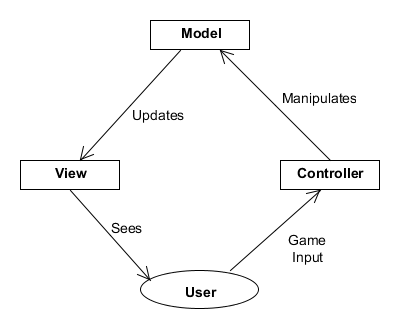
\includegraphics[scale=0.5]{images/MVC.png}}
    \caption{Model-View-Controller within a game context.}
    \label{fig:mvc}
\end{figure}
\subsection{Design class diagram}
\label{ss:design-class-diagram}
The design class digram is too large to fit into an A4 page, it is therefore a separate document: \textit{\textbf{Appendix A - DesignClassDiagram.pdf}}. The class diagram is extensive and highly detailed and shows the relationships between the classes. It also captures the hierarchy between classes. The following is a description of the notation used within the class diagram:
\begin{center}
    \begin{tabular}{|c|c|}
        \hline
        \textbf{Symbol} & \textbf{Description} \\
        \hline
        + & Public \\
        \textasciitilde  & Internal \\
        - & Private \\
        underline & Static \\
        italic & Abstract \\
        \hline
    \end{tabular}    
\end{center}
\subsection{Layered architecture}
The game is build upon the Unity engine. It forms the core or foundation layer of the system. The Unity engine provides functionality for physics calculations, controlling animations, rendering the scene, lighting calculations and collision detection to name a few. No technical services layer was included as the game does not have application-independent services such as connections to databases or extensive logging of errors to file. This layer will be added if in a later iteration a use case that requires such services is developed. The layer above that is the domain layer. It holds software objects representing domain concepts that fulfill application requirements. The majority of the classes belong to this layer since they are specific to the context of this game. At the topmost layer lies the user interface layer. It is highly specific to the application and contains services that the user will interact with. Such services include the world, menus and heads-up display.\smallskip\\
The game makes use of a relaxed layered architecture as the both the user interface layer and domain layer call the engine layer directly. It was decided that a strict layered architecture was inadvisable. The performance impact would be far too high. In a game, the performance is a primary concern. Secondly, it would require a wrapper in the domain layer to allow commands to be passed from the user interface through to the engine layer which would be time consuming to develop. \smallskip\\
In this game, the world and level design is a critical factor. It is therefore important to identify where it belongs within the architecture of the system in order to see how changes to it would effect the system as a whole. It was identified that the world should belong to the user interface layer. This is justified as the user can see and interact with the world just as they would see and interact with a web page. The world is therefore classified the same as one would classify the HyperText Markup Language (HTML) and Cascading Style Sheets (CSS) of a web page. The result is that one can make aesthetic changes and changes to the layout of the level without affecting any other part of the system.
\begin{figure}[H]
    \center{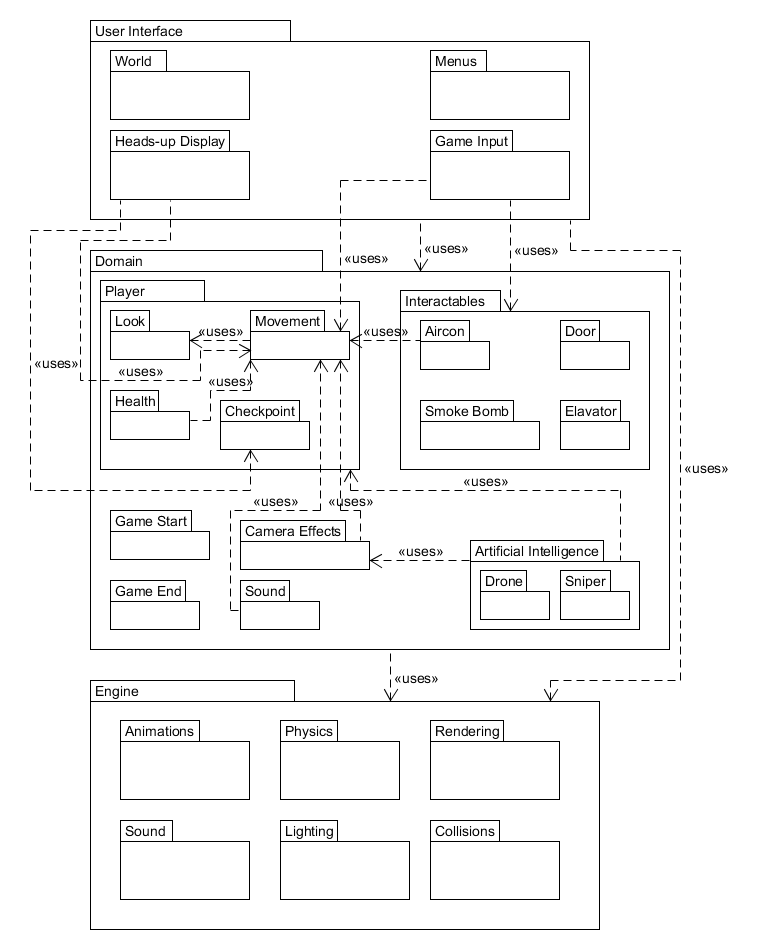
\includegraphics[scale=0.7]{images/LayeredArchitectureDiagram.png}}
    \caption{Architecture of the game}
    \label{fig:architecture}
\end{figure}
\subsection{Data organisation}
The system does not make use of any explicit databases or output to text files. However, since the Unity engine is used it it important to ensure that the data type of the assets used was one which the engine provided support for. The classes were written in C\#, models (possibly with animations) in the fbx format, textures as a png image and materials as a mat file.\smallskip\\
The folder structure of the assets need to be well structured and easy to manage to allow the game to scale. A folder for art assets from the artists is used, each asset is then separated into a different folder. Each asset folder has the texture, fbx and materials. Fonts, other materials defined, prefabs, scenes, shaders, sound and standard assets are defined to their own folder. A folder called scripts is used to store all the classes. The scripts folder structure is the same as that defined in figure \ref{fig:architecture}.\smallskip\\
The algorithms used will be covered in detail in section \ref{s:implementation} and will not be covered in this section.

\section{Implementation}
\label{s:implementation}
\subsection{Player Controller}
\subsubsection{Re-usability and encapsulation}
Since the game must support two independent players, a large amount of code duplication is possible in supporting the interaction of the various game systems with both players. Extensive use of the engine's built-in object-component model is used to write instance-independent scripts that will handle the relevant interactions with the world and then attach them to each player object. \\
This results in each player object functioning entirely independently, meaning that not only can we support extra players by placing extra player avatars in the world, but bugs and code modifications only occur once and the changes apply to both players.
\subsubsection{Camera control}
Control of the player's camera is handled by two different scripts, one for rotation in each of the X and Y axes. This separation of axes is useful because while the rotation in the X axis needs to rotate only the camera (to allow the player to look up or down), the rotation about the Y axis also needs to rotate the entire player object (containing the camera, the 3D model, all attached scripts etc). \\
In both the X and Y cases, the script gets the relevant player's input for that frame and then rotates itself appropriately.
\subsubsection{Input separation}
Having multiple players over a network is not supported so both players must play on the same computer. A way is therefore needed to separate the input for either player so that player one does not respond to input intended for player two (for example). This separation is achieved by inserting an extra layer of abstraction between the code that handles player input, and the engine which acquires that input from the operating system/hardware. \\
Instead of asking the engine for the state of input directly, the player scripts ask the "InputSplitter" class for the state of player input for only that player, InputSplitter then handles all separation of input invisibly and only gives back the appropriate commands.
\subsubsection{Environment interaction}
Environment interaction forms the bulk of the code for the player controller. The player needs to be able to complete a number of distinct actions, namely: running, jumping, sliding, climbing and vaulting. All of these actions require separate handling. Fortunately the transitions between these actions are fairly clear and well-defined. A finite state machine solution is used. \\
The player's default state is "Idle", where the player is simply standing still and not moving around at all. One can even consider this to be the same state as the player's next most common state: "Running" (since idling can be thought of as simply running with a speed of zero). Running is also the state with the most complicated situation regarding state transitions since all the other states transition in and out of  the running state. \\
While in the running state, the player can change state either by pressing the jump button, or pressing the slide button. When the slide button is pressed the player will go into a low slide across the ground, as long as they are moving fast enough in the first place. This slide will cause the player to slow down over time (which enforces a limit on how far the player can slide) but will allow them to move beneath low-hanging objects and possibly move around the level in an overall smoother or faster fashion. \\
If the player presses the jump button, the controller first needs to examine the player's surroundings to see what obstacles there are. If there is a low obstacle on the floor in front of the player, then the player will either climb onto it if they are currently stationary, or vault over it if they are moving. If there is an obstacle in front of the player that is too tall to vault over, but not tall enough that the player cannot reach the top of it, then the player will climb up onto the obstacle. If no such obstacles are present, the player will simply jump.
\begin{figure}[H]
    \center{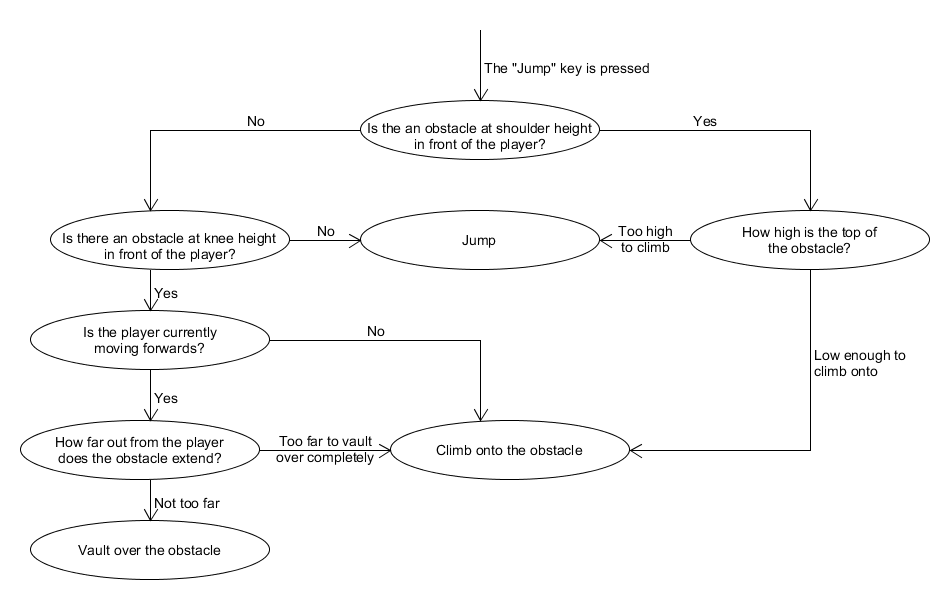
\includegraphics[scale=0.4]{images/JumpDecisionTree.png}}
    \caption{The decision tree that plays out when the player presses the "jump" key}
    \label{fig:jumpDecisionTree}
\end{figure}
In order to facilitate this process of checking the player's surroundings, we make extensive use of the engine's built in physics systems that allow code to easily shoot a ray through the world and provide information about what (if anything) the ray hits. Such a ray cast is used to check for the existence of obstacles at various heights in front of the player, as well as how far upwards those objects extend. \\
\begin{figure}[H]
    \center{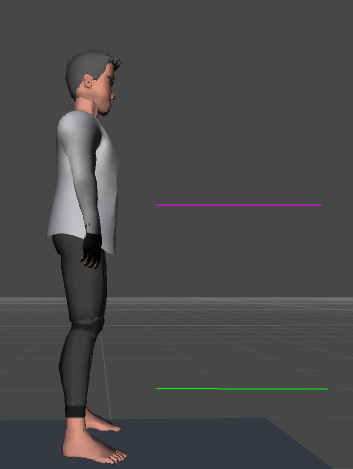
\includegraphics[scale=0.5]{images/raycastHeights.png}}
    \caption{The player avatar with the obstacle check heights for low (green) and tall (pink) obstacles }
    \label{fig:raycastCheckHeights}
\end{figure}
\subsubsection{Issues encountered}
The main issue encountered while developing the code for controlling the player character is that the code would incorrectly classify the situation when the player pressed the "jump" key and would for example try to climb onto an obstacle that should have been vaulted over. This was mostly caused by badly tuned parameters for deciding at which height obstacles should be checked for, but was also caused by things such as having very thin pieces of world geometry that the system could fail to detect, resulting in incorrect behaviour. \\
The other common issue was that when vaulting, climbing or sliding, the player would clip into world geometry and get stuck. This was a result of those motions failing to correctly make use of the engines physics systems, causing the player to move into geometry and then find themselves stuck when control was returned to the default code for running around. Once again, fixing these issues mostly involved ensuring that the engine's physics state is correctly updated in all the appropriate places while the player is moving.
\subsection{Configurable agents}
In order to create a game that is balanced and fun to play, requires agents that are highly configurable. Unity provides an interface to configure class variables within the editor and while the game is running. This feature is leveraged to create configurable agents. An additional benefit this brings is that AI agents can be configured on the micro (per agent) level. It allows the level designer the ability to control the risk-reward ratio of the various routes which the player can take. Secondly, it provides a means to the level designer to be able to nudge the player towards certain desired behaviour. An example of the aforementioned is snipers which have been placed next to the first passage within the game. They are placed in order to encourage the player to slide below each window. 
\subsection{Drone}
\subsubsection{Introduction}
The drone has four distinct states which it can be in at any given time: avoiding obstacle, patrolling, chasing and shooting. The logic used to determine what state the drone is in at any given time is shown in figure \ref{fig:droneDesisionTree}.
\subsubsection{Obstacle avoidance}
The drone makes use of a basic obstacle avoidance algorithm. It ray-casts forward 10 units and does a second ray-cast downwards 2 units. If either ray-cast hits an object which it deems it should avoid it will move upwards every game cycle until it no longer hits an object. The drone can then move forward over the obstacle. In the level design stage it was declared that drones are always used in open areas and that the area above them is always free. As such this simple straightforward algorithm was used as it is not necessary to use a more complex technique to achieve the desired behaviour.
\subsubsection{Patrolling}
Patrolling is the default state of the drone. Each drone has a set of way-points that it faces and moves towards. The drone may only move towards its destination if it is within two degrees of facing the destination. Once the drone reaches its destination the next waypoint is set as the destination. If all the way-points are consumed the index is reset and the destination is set to the start of the list. The data structure used here is an array of Vector3's. The Vector3 represents the position in the game world that the drone should move towards. An array was used as it has O(1) access and because the number of way-points are static at runtime.
\subsubsection{Chasing}
Chasing occurs when a player triggers the drone's detection sphere causing the last seen position variable to be updated to a non-default value. Only one player can be targeted at a given time. Within the chasing state the drone maintains the position that the player was last seen as a Vector3. This position is updated at every game tick that the player is still triggering the detection sphere. If the drone loses sight of the player, it will move towards the last seen position. A timer starts that keeps track how long the drone has lost sight of the player for. If this timer exceeds the defined threshold (currently five seconds) then the drone's state is reset. If the drone detects a player while moving towards the last known position then that player will become tracked.
\subsubsection{Shooting}
Shooting occurs if the player is tracked and the drone is facing towards the player. To keep the drone interesting and to add some variation the drone employs an offset function which offsets the bullet trajectory. The offset function is a summation of three sub-functions which each use different input variables to calculate their offset. Figure \ref{fig:offset} is a graph depicting the input and output for each sub-function (note that the second and third offsets use the same function but take different input).\smallskip\\
The first sub-function takes the time the player has been tracked by the drone as input. It uses an exponential decay function so the offset rapidly decreases the longer the player is tracked. The second sub-function takes the movement speed of the player as input. It uses a linear function to compute the offset. If the player stays moving the probability of getting hit is slightly less. The third sub-function takes the distance from the player into account. Players that are close to the edge of the detection sphere are less likely to be hit then those who run through under the drone.\smallskip\\ 
The constants for each function were found through play testing and through consultation with the level designer as to the desired accuracy. Through play-testing the initial constants were dramatically reduced to their current values. The exponential decay function started at an initial value too high. The movement offset was also too high and caused drone to miss all their shots as long as the player kept moving. 
\begin{figure}[H]
    \center{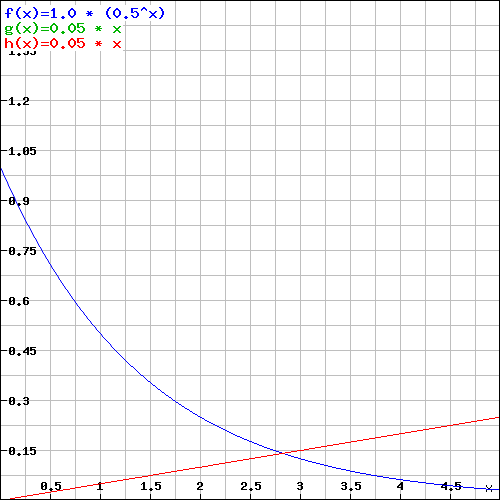
\includegraphics[scale=0.65]{images/offset_graph.png}}
    \caption{Plot of the offset functions where x is the input to the function and y is the offset}
    \label{fig:offset}
\end{figure}
\begin{figure}[H]
    \center{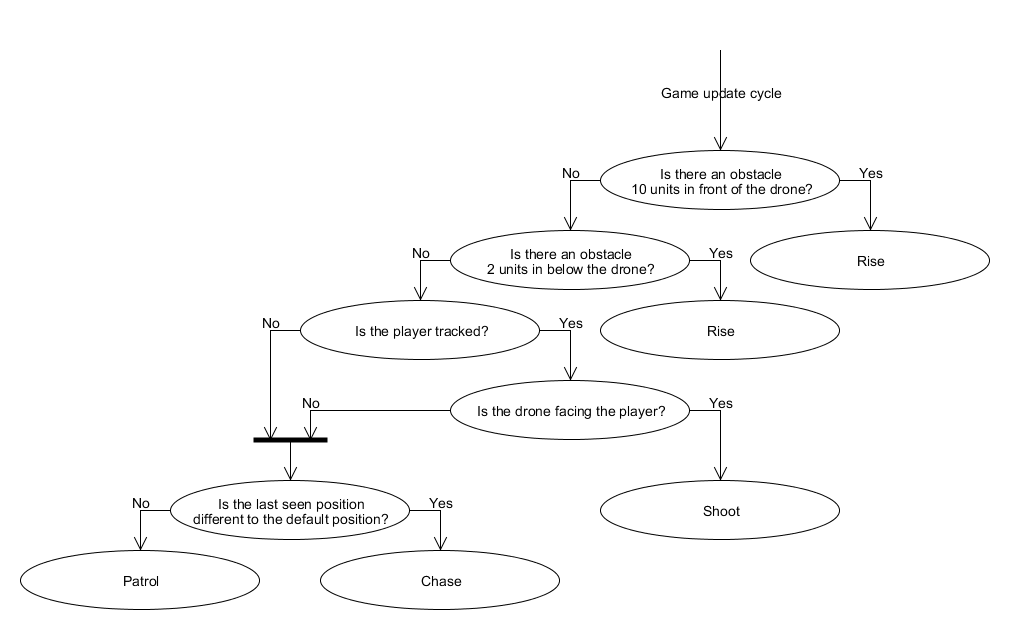
\includegraphics[scale=0.5]{images/DroneDecisionTree.png}}
    \caption{Decision tree for drone that plays out each game update cycle}
    \label{fig:droneDesisionTree}
\end{figure}
\subsection{Sniper}
\subsubsection{Introduction}
Sniper has three distinct states that it can be in at any given time: patrolling, chasing and shooting. The sniper activates using triggers placed in the environment. The logic behind the transitions between sniper states is depicted in figure \ref{fig:sniperDecisionTree}.
\subsubsection{Patrolling}
Patrolling is the default state of the sniper. The sniper tracks to a random position at the bottom of the trigger. Once the sniper reaches the random position a new random position is calculated. A ray-cast is done to calculate the length of the laser up to 1000 game units. Since the laser extends into the environment it means only the rotation of the laser needs to change at each game update cycle.
\subsubsection{Chasing}
When a player enters a trigger monitored by the sniper, there is a configurable delay until they become tracked. Once tracked, the laser moves towards the player.
\subsubsection{Shooting}
Shooting occurs when the player is tracked and the laser is pointing towards the player. There is a configurable delay before each bullet is fired. This is achieved using a simple timer that is updated at each game update cycle. The shoot timer is purposefully not reset when the sniper targets another player. This allows cunning players to decrease the timer such that the sniper cannot shoot yet but will be able to shoot near instantly if the player behind enters that sniper's trigger area. While many of the mechanics in the game offer ways for the player behind to catch up, this offers a means for the player ahead to maintain their lead.
\begin{figure}[H]
    \center{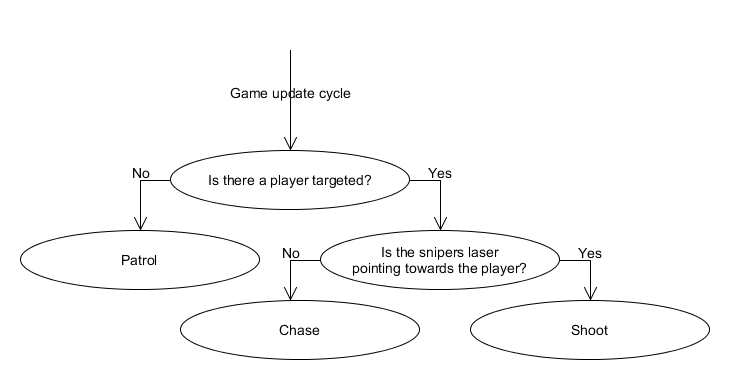
\includegraphics[scale=0.5]{images/SniperDecisionTree.png}}
    \caption{Decision tree for sniper that plays out each game update cycle}
    \label{fig:sniperDecisionTree}
\end{figure}
\subsection{Heads-up display (HUD)}
\subsubsection{Dynamic movement}
\label{sss:dynamic_movement}
The heads-up display uses a simple algorithm to move its position back and forth on the screen. The class uses two defined variables, the time to swap and the movement per time increment. Every game update cycle the timer updates and the heads-up display moves some increment if a condition is met. The condition is that the player is moving and is on the ground and is not in a context specific jump action. This limits updates to when the player is running on the ground where it is intended. When the timer exceeds the set threshold, the direction of movement is reversed - creating a rocking motion.
\subsubsection{Position}
The position indicator gives the player an indication of what position they are in the race. The algorithm for the position in the race is calculated as follows: if player one has passed more checkpoints than player two then player one is in the lead. Similarly, if player two has passed more checkpoints than player one then player two is in the lead. When the number of checkpoints are equal then the linear distance to the next checkpoint is used. This can lead to some inaccuracies since the the map is not linear in nature. This inaccuracy is noticeable in the bowl-shaped section of the level. To develop a more accurate measure would require a complex algorithm and many hours of work which were not available to complete this use case. The level of error from the algorithm has been deemed acceptable by the development team and from play testing is not particularly noticeable.
\subsection{Checkpoints}
Checkpoints are implemented as colliders within the level. A set (implemented as a hash-table) containing positions of checkpoints is used to check if a checkpoint reached has already been reached in the past. If the player has not reached the checkpoint before, which is checked by looking up the position of the checkpoint in the set, then the position of the checkpoint is added to the set. If the position exists in the set when the player reaches the checkpoint then no action is taken. A hash-table was used because it provides O(1) lookup and O(1) insertion for the average case. It is therefore very efficient. 
\subsection{Health}
\subsubsection{Player health}
The player starts with a finite health value. When the player is damaged their health is reduced. When the player's health is zero or less then the player is killed. The player health class uses a configurable variable for the time it takes to start healing after taking damage and the rate at which the player is healed at. A timer is set to 0 when the player takes damage and is incremented by the change in time at each game update cycle while the player is not at full health. This timer is used to indicate when the player can start regenerating heath. A float is used to store the time as the change in time is stored as a float in Unity. It is also not necessary to have the floating point precision of a double (which would require more memory) for this task.
\subsubsection{Player Re-spawn}
\label{sss:re-spawn}
When a player is killed the screen fades to black  at a set rate. Once the screen has faded to black, the player is re-spawned at the last checkpoint passed. Once re-spawned, the screen then clears at a set rate. The player can be killed from a method call, for example the health class will call kill when the player's health is less than or equal to zero. The player movement class can call kill if the player landed at a velocity that exceeds a set threshold. This class itself will kill the player if their vertical velocity exceeds a set threshold, this is used to re-spawn players who have fallen off the map.
\subsection{Camera effects}
\subsubsection{Headbob}
Headbob is implemented exactly the same as described in section \ref{sss:dynamic_movement} except that headbob moves the camera vertically and dynamic movement moves the HUD horizontally. Headbob uses different configuration variables than dynamic HUD but the basic algorithm remains the same.
\subsubsection{Hit flash}
Hit flash uses a similar algorithm to that of section \ref{sss:re-spawn}. When a player is hit by a bullet from the AI the flash camera method of hit flash is called. Instead of fading to black and then clearing as with re-spawning, the flash camera method sets the screen immediately black and then rapidly clears.
\subsection{Interactables}
\subsubsection{Introduction}
All interactables include an activation function that start some defined behaviour.
\subsubsection{Air conditioning}
When the air conditioning is activated via the terminal, it releases steam in the trench. This steam slows the player down. This is implemented via a collider. Activating the terminal makes the air conditioning fan rotate, plays a steam particle effect and activates the player slow script. When a player comes in contact with a collider their run speed is decreased linearly to a set value. When they leave the collider their run speed is increased linearly back to the default run speed. The rate the player decelerates is much greater than the rate that they accelerate when they exit the collider. The result is that players lose valuable time. While this route is safe from drones, it can also be countered by the opponent if they see that the other player is moving towards the trench.
\subsubsection{Elevator}
In the start-up method of the elevator it calculates the distance that the elevator must drop to reach the floor below. When the player presses the terminal in the elevator, the elevator starts moving downwards at a set velocity until it reaches the floor. The elevator door closes when the player uses the elevator, this prevents the other player being able to use it but also indicates to the other player that the elevator has been used. That player can then activate another terminal in the area that slows the elevator down by a large factor (currently five times slower) for a few seconds. It also releases sparks from above to obstruct the players view and indicate to the player inside the elevator that they have been slowed. A timer is used to calculate how long the elevator has been slowed for. Once this timer is exceeded, the elevator resumes at regular speed.
\subsubsection{Smoke bomb}
When the smoke bomb input is given, an animation plays which throws the smoke bomb to the ground. When the bomb hits the ground a smoke cloud particle effect plays. Associated with that is a sphere collider that expands for up to 6 seconds with the radius growing at a rate of 0.5 units times the change in time between the update cycle. The AI cannot target a player through the smoke bomb, allowing the player to escape. The player is only given two smoke bombs for the level so the player has to chose wisely when to use theirs.
\section{Program Validation and Verification}

\begin{table}[H]
\caption{Testing Plan Summary}
	\begin{center}
		\begin{tabular}{ |l|p{10cm}| } 
			\hline
			Process & Technique \\ \hline
			Integration Testing & Placed various game components in the game world together and tested whether they interacted correctly with each other. \\ \hline
			Validation Testing & Tested various use cases relating to game mechanics by repetitive play testing of the game. \\ \hline
			User Tests & Asked volunteers to play through the game and comment on various aspects of gameplay such as look and feel.\\
			\hline
		\end{tabular}
	\end{center}
\end{table}
These testing techniques were chosen as they are suitable to test interactive 3D games designed in Unity. Integration testing allowed us to test individual game elemnts in the enviroment they would be used in as well as allowing us to gradually build up smaller components into larger ones which were then tested via validation testing. Validation testing lends itself to intensive play testing which is suitable to testing games. Below there is an extensive record of how we tested a wide variety of possible use cases in order to ensure all apsects of our game worked as intended. User Tests were implemented as it is often impossible for game designers to judge certain aspects of their own game such as how intuitive the controls are. They also allow us to do a larger number of play tests as we are able to utilize a larger testing population.
\begin{table}[H]
	\caption{Validation Tests Summary}
	\begin{center}
		\begin{tabular}{ |c|c|c|c| } 
			\hline
			Test Type & \multicolumn{3}{|c|}{Test Result}\\ \hline
			& Functional Tests & Animation Tests & Rendering Test\\ \hline
			Movement Tests & Passed & Passed & n/a\\ \hline
			Look Tests & Passed & Failed & n/a\\ \hline
			Vault Tests & Failed & Failed & n/a\\ \hline
			Jump Tests & Passed & Failed & n/a\\ \hline
			Climb Tests & Passed & Passed & n/a\\ \hline
			Slide Tests & Passed & Passed & n/a\\ \hline
			Ledge Grab Tests & Failed & Failed & n/a\\ \hline
			Smokebomb Tests & Passed & Passed & Passed\\ \hline
			Re-spawn Tests & Passed & n/a & Passed\\ \hline
			Checkpoint Tests & Passed & n/a & n/a\\ \hline
			Vent Tests & Passed & n/a & Passed\\ \hline
			Elevator Tests & Passed & n/a & Passed\\ \hline
			Door Tests & Passed & n/a & Passed\\ \hline
			Drone Tests & Passed & Passed & Passed\\ \hline
			Sniper Tests & Passed & n/a & Passed\\ \hline
			UI Tests & Passed & n/a & Passed\\ \hline
		\end{tabular}
	\end{center}
\end{table}

%I Copy-pasted my cases from Stage 3
%This needs to be expanded quite a lot as it does not cover all the cases e.g. missing cases are ones for elevator (ands its interactions with slow button), door, smokebomb (it only has 2 charges!, its interactions with AI), position in the race (UI), the ledge grap, All of AI interactions many possible cases can be thought up there.
\subsection{Integration Tests}
%Direct input to function call tests seem to belong here, possibly will add some AI-World interaction tests here too
\subsubsection{Keyboard/Mouse Input}
\textbf{Tests prepared} \\
Description: Mouse calls correct player look functions.\\
Expected Result: Player look function called on mouse input.\\
Actual Result: As expected.\\
Status: Pass
\smallskip\\
Description: WASD keys calls correct player movement functions.\\
Expected Result: Player movement function called on key press.\\
Actual Result: As expected.\\
Status: Pass
\smallskip\\
Description: Spacebar key calls player jump function.\\
Expected Result: Player jump function called on key press.\\
Actual Result: As expected.\\
Status: Pass
\smallskip\\
Description: Shift key calls correct player slide function.\\
Expected Result: Player slide function called on key press.\\
Actual Result: As expected.\\
Status: Pass
\smallskip\\
Description: F key calls correct deploy smokebomb function.\\
Expected Result: Use smokebomb function called on key press.\\
Actual Result: As expected.\\
Status: Pass
\smallskip\\
Description: E key calls door open function if used by player near a door\\
Expected Result: Door open function called on key press.\\
Actual Result: As expected.\\
Status: Pass
\smallskip\\
Description: E key calls button function if used by player near a unused button\\
Expected Result: Button function called on key press.\\
Actual Result: As expected.\\
Status: Pass
\subsubsection{Controller Input}
\textbf{Tests prepared} \\
Description: Right Joystick calls correct player look functions.\\
Expected Result: Player look function called on right joystick input.\\
Actual Result: As expected.\\
Status: Pass
\smallskip\\
Description: Left Joystick calls correct player movement functions.\\
Expected Result: Player movement function called on left joystick input.\\
Actual Result: As expected.\\
Status: Pass
\smallskip\\
Description: Left bumper calls player jump function.\\
Expected Result: Player jump function called on left bumper press.\\
Actual Result: As expected.\\
Status: Pass
\smallskip\\
Description: Right bumper key called correct player slide function.\\
Expected Result: Player slide function called on right bumper press.\\
Actual Result: As expected.\\
Status: Pass
\smallskip\\
Description: B button press calls correct deploy smokebomb function.\\
Expected Result: Use smokebomb function called on B button press.\\
Actual Result: As expected.\\
Status: Pass
\smallskip\\
Description: A button calls door open function if used by player near a door\\
Expected Result: Door open function called on A button press.\\
Actual Result: As expected.\\
Status: Pass
\smallskip\\
Description: A button key calls button function if used by player near a unused button\\
Expected Result: Button function called on A button press.\\
Actual Result: As expected.\\
Status: Pass
\subsection{Validation Tests}
%This section is mostly complete will add some more multiplayer specific tests once more multi-player testing has happened
\subsubsection{Movement}
\textbf{Tests prepared}\\
Description: Move player forward with no obstruction in the given direction.\\
Expected Result: Player moves forward at the speed configured.\\
Actual Result: As expected.\\
Status: Pass
\smallskip\\
Description: Move player left with no obstruction in the given direction.\\
Expected Result: Player moves left at the speed configured.\\
Actual Result: As expected.\\
Status: Pass
\smallskip\\
Description: Move player right with no obstruction in the given direction.\\
Expected Result: Player moves right at the speed configured.\\
Actual Result: As expected.\\
Status: Pass
\smallskip\\
Description: Move player backwards with no obstruction in the given direction.\\
Expected Result: Player moves backwards at the speed configured.\\
Actual Result: As expected.\\
Status: Pass
\smallskip\\
Description: Move player forwards with an obstruction in the given direction.\\
Expected Result: Player moves forwards at the speed configured until its collider connects with the obstruction, the player can then no longer move forward.\\
Actual Result: As expected.\\
Status: Pass
\smallskip\\
Description: Move player left with an obstruction in the given direction.\\
Expected Result: Player moves left at the speed configured until its collider connects with the obstruction, the player can then no longer move left.\\
Actual Result: As expected.\\
Status: Pass
\smallskip\\
Description: Move player right with an obstruction in the given direction.\\
Expected Result: Player moves right at the speed configured until its collider connects with the obstruction, the player can then no longer move right.\\
Actual Result: As expected.\\
Status: Pass
\smallskip\\
Description: Move player backwards with an obstruction in the given direction.\\
Expected Result: Player moves backwards at the speed configured until its collider connects with the obstruction, the player can then no longer move backwards.\\
Actual Result: As expected.\\
Status: Pass
\smallskip\\
Description: Run animation plays in direction of movement.\\
Expected Result: The run animation plays and makes player model look as if it is running in the given direction\\
Actual Result: As expected\\
Status: Pass
\subsubsection{Look}
\textbf{Tests prepared}\\
Description: Player can can turn full 360 degrees horizontally\\
Expected Result: Players view turns horizontally by a configurable angle in the direction of the horizontal mouse movement.\\
Actual Result: As expected.\\
Status: Pass
\smallskip\\
Description: Player can can turn head up to a bounded angle vertically\\
Expected Result: Player view turns vertically by a configurable angle in the direction of the vertical mouse movement. The players vertical view angle is prevented from exceeding the defined range\\
Actual Result: As expected.\\
Status: Pass
\smallskip\\
Description: Player head faces direction of look\\
Expected Result: Player head looks in the direction of the view.\\
Actual Result:  Head remains static.\\
Status: Failure
\subsubsection{Vault}
\textbf{Tests prepared}\\
Description: Player can vault over object that is less than 1 metre high and has a length that is less than 3 metres and is moving at least 5 metres per second. \\
Expected Result: Player vaults over object.\\
Actual Result:  As expected.\\
Status: Pass
\smallskip\\
Description: Player can not vault over object that is less than 1 metre high and a length that is more than 3 metres or is moving at less than 5 metres per second. \\
Expected Result: Player climbs onto object.\\
Actual Result:  Player is moved up and onto the object but with excessive velocity that projects them further.\\
Status: Failure
\smallskip\\
Description: Player can not vault over object that is more than 1 metre high\\
Expected Result: Player initiates a climb if it meets the climb parameters else initiates a jump.\\
Actual Result: As expected.\\
Status: Pass
\smallskip\\
Description: Player vault animation plays if vault action initiated\\
Expected Result: The vault animation plays and makes the model look as if it is vaulting over the object.\\
Actual Result:  No animation plays.\\
Status: Failure
\subsubsection{Jump}
\textbf{Tests prepared}\\
Description: The player jumps upwards if no other contextual action available and player is stationary. \\
Expected Result: Player jumps upwards.\\
Actual Result:  As expected.\\
Status: Pass
\smallskip\\
Description: The player jumps in direction of motion if no other contextual action available and player is moving. \\
Expected Result: Player jumps in direction of motion.\\
Actual Result: As expected.\\
Status: Pass
\smallskip\\
Description: The player jump animation plays if player jumps. \\
Expected Result: Jump animation plays.\\
Actual Result:  No animation plays.\\
Status: Failure
\subsubsection{Climb}
\textbf{Tests prepared}\\
Description: The player climbs the object in front of it if it is unable to initiate a vault on the object and it is less than 3.05 metres tall. \\
Expected Result: Player climbs object.\\
Actual Result: As expected.\\
Status: Pass
\smallskip\\
Description: The player climbs animation plays during a climb. \\
Expected Result: Climb animation plays.\\
Actual Result:  As Expected.\\
Status: Pass
\subsubsection{Slide}
\textbf{Tests prepared}\\
Description: Slide can only be initiated when the player is grounded and is not in a different action\\
Expected Result: Player slides.\\
Actual Result: As expected.\\
Status: Pass
\smallskip\\
Description: Slide decreases player velocity at a defined rate. \\
Expected Result: Player slows down during slide.\\
Actual Result: As expected.\\
Status: Pass
\smallskip\\
Description: Slide can only be initiated if player is moving above a defined amount. \\
Expected Result: Player slides if moving above defined amount. Else, player does not slide\\
Actual Result: As expected.\\
Status: Pass
\smallskip\\
Description: Slide animation plays if a slide is initiated. \\
Expected Result: Player slide animation plays which makes the model look as if it is sliding.\\
Actual Result: As Expected.\\
Status: Pass
\subsubsection{Ledge Grab}
\textbf{Tests prepared}\\
Description: The player hits an obstacle in front of them while not grounded and the obstacle does not extend above the player's head.\\
Expected Result: Player drops down to hanging position and then climbs onto obstacle.\\
Actual Result: Player climbs onto obstacle.\\
Status: Failure
\smallskip\\
Description: The player hits an obstacle in front of them while not grounded and the obstacle extends above the player's head. \\
Expected Result: Player falls down.\\
Actual Result: As expected.\\
Status: Pass
\smallskip\\
Description: The player hits an obstacle in front of them while grounded and the obstacle does not extend above the player's head. \\
Expected Result: Player forward movement halts\\
Actual Result: As expected.\\
Status: Pass
\smallskip\\
Description: Player should be animated to show the ledge grab and following climb\\
Expected Result: Player animates to hanging position and then plays climbing animation\\
Actual Result: Player Climbing animation plays\\
Status: Failure
\subsubsection{Smokebomb}
\textbf{Tests prepared}\\
Description: The player uses a smokebomb with smokebombs available\\
Expected Result: Small collider is created and raycasts do not detect the player character for 2 seconds\\
Actual Result: As expected.\\
Status: Pass
\smallskip\\
Description: The player uses a smokebomb with no smokebombs available \\
Expected Result: Nothing occurs\\
Actual Result: As expected.\\
Status: Pass
\smallskip\\
Description: A smokebomb is used \\
Expected Result: Smokebomb particle effects rendered in the world\\
Actual Result: As expected.\\
Status: Pass
\smallskip\\
Description: Player should be animated to show a downward throwing action\\
Expected Result: Throwing animation plays on successfull use of smokebomb\\
Actual Result: As Expected\\
Status: Pass
\subsubsection{Re-spawn}
\textbf{Tests prepared}\\
Description: Screen dims when the velocity the player is falling at a defined rate\\
Expected Result: Screen starts to dim.\\
Actual Result: As expected.\\
Status: Pass
\smallskip\\
Description: Screen clears when the velocity the player is not falling at a defined rate\\
Expected Result: Screen starts to clear.\\
Actual Result: As expected.\\
Status: Pass
\smallskip\\
Description: Player re-spawns when the screen dims beyond a defined amount\\
Expected Result: Player re-spawns at last checkpoint reached and screen clears.\\
Actual Result: As expected.\\
Status: Pass
\subsubsection{Checkpoints}
\textbf{Tests prepared}\\
Description: Latest checkpoint updates if the players reaches a checkpoint not in set of checkpoints reached.\\
Expected Result: Latest checkpoint set as the current checkpoint reached.\\
Actual Result: As expected.\\
Status: Pass
\smallskip\\
Description: Latest checkpoint does not update if the players reaches a checkpoint already in set of checkpoints reached.\\
Expected Result: No change to system.\\
Actual Result: As expected.\\
Status: Pass
\subsubsection{Aircon vent expels steam to slow player}
\textbf{Tests prepared}\\
Description: Player only slowed when the aircon is active.\\
Expected Result: Player is slowed.\\
Actual Result: As expected.\\
Status: Pass
\smallskip\\
Description: Steam only shows if aircon is active.\\
Expected Result: Steam effect expelled from aircon vent.\\
Actual Result: As expected.\\
Status: Pass
\smallskip\\
Description: Player is not slowed when the aircon is not active.\\
Expected Result: Player is not slowed.\\
Actual Result: As expected.\\
Status: Pass
\subsubsection{Elevator}
\textbf{Tests prepared}\\
Description: Elevator moves down when elevator button is pressed.\\
Expected Result: Elevator floor descends.\\
Actual Result: As expected.\\
Status: Pass
\smallskip\\
Description: Elevator door closes when elevator button is pressed..\\
Expected Result: Door moves up.\\
Actual Result: As expected.\\
Status: Pass
\smallskip\\
Description: Elevator is slowed when elevator sabotage button is pressed\\
Expected Result: Elavator floor descends more slowly for 2 seconds.\\
Actual Result: As expected.\\
Status: Pass
\smallskip\\
Description: Particles effect plays when elevator sabotage button is pressed\\
Expected Result: Particles are rendered and fall down elevator shaft.\\
Actual Result: As expected.\\
Status: Pass
\subsubsection{Door}
\textbf{Tests prepared}\\
Description: Door opens when player presses action button while near it and it is closed.\\
Expected Result: Door opens.\\
Actual Result: As expected.\\
Status: Pass
\smallskip\\
Description: Door does nothing when player presses action button while near it and it is open.\\
Expected Result: No result.\\
Actual Result: As expected.\\
Status: Pass
\smallskip\\
Description: Door prevents player from moving through doorway while closed.\\
Expected Result: Player collides with door.\\
Actual Result: As expected.\\
Status: Pass
\smallskip\\
Description: Door allows player from moving through doorway while open.\\
Expected Result: Player moves through doorway.\\
Actual Result: As expected.\\
Status: Pass
\smallskip\\
Description: Door is rendered correctly while open/closed\\
Expected Result: Door is rendered in all states.\\
Actual Result: As expected.\\
Status: Pass
\subsubsection{Drone}
\textbf{Tests prepared}\\
Description: Drone patrols between checkpoints when no players are close and visible.\\
Expected Result: Drone patrols between checkpoints.\\
Actual Result: As expected.\\
Status: Pass
\smallskip\\
Description: Drone moves toward players that are close and visible.\\
Expected Result: Drone moves toward player.\\
Actual Result: As expected.\\
Status: Pass
\smallskip\\
Description: Drone shoots players that are sufficiently close and targeted and in sight.\\
Expected Result: Drone shoots targeted player and player loses health.\\
Actual Result: As expected.\\
Status: Pass
\smallskip\\
Description: Drone does not shoot players that are sufficiently close and targeted and not in sight.\\
Expected Result: Drone moves to location the player was last visible at.\\
Actual Result: As expected.\\
Status: Pass
\smallskip\\
Description: Drone avoids obstacles in it's path while chasing players or patrolling\\
Expected Result: Drone flies over any obstacles it encounters.\\
Actual Result: As expected.\\
Status: Pass
\subsubsection{Sniper}
\textbf{Tests prepared}\\
Description: Sniper targets random locations at the bottom of sniper colliders while there are no players in any of the colliders assigned to the sniper\\
Expected Result: Sniper laser moves around the bottom of sniper colliders.\\
Actual Result: As expected.\\
Status: Pass
\smallskip\\
Description: Sniper targets players in its colliders that are visible after a set amount of time.\\
Expected Result: After a player has been in a sniper's collider and visible for some time the sniper will turn towards the player and shoot him\\
Actual Result: As expected.\\
Status: Pass
\smallskip\\
Description: Sniper will stop targeting the player as soon as he exits the sniper collider or is not in line of sight.\\
Expected Result: Sniper returns to passive mode.\\
Actual Result: As expected.\\
Status: Pass
\subsubsection{UI}
\textbf{Tests prepared}\\
Description: Headbob occurs only while the player is moving\\
Expected Result: Headbob occurs while the player is moving, headbob does not occur while the player is not moving\\
Actual Result: As expected.\\
Status: Pass
\smallskip\\
Description: Player position is accurately reflected in the UI.\\
Expected Result: Player position should be 1 of 2 if the player is ahead of the other player and 2 of 2 otherwise\\
Actual Result: As expected.\\
Status: Pass
\smallskip\\
Description: Time should be accurately displayed by the UI.\\
Expected Result: Time should start at 0:00 and be incremented to match real time passed since the game started.\\
Actual Result: As expected.\\
Status: Pass
\subsection {User Testing}
%Will add to this section once I get some more user tests
A variety of users were asked to play the game on both controller and mouse/keyboard input methods. Players were then asked to rank the following game-play aspects on a scale of 1 to 5 with 1 being very bad and 5 being very good; Controls, Flow, Visuals, Sound, Multi-player and Fun. Users were also asked to provide comments on aspects of the game that caught their attention whether positive or negative. Below is a graph showing the average rating of each aspect of the game that users ranked. Included is a list of comments that were common amongst a variety of users.
\begin{figure}[H]
	\center{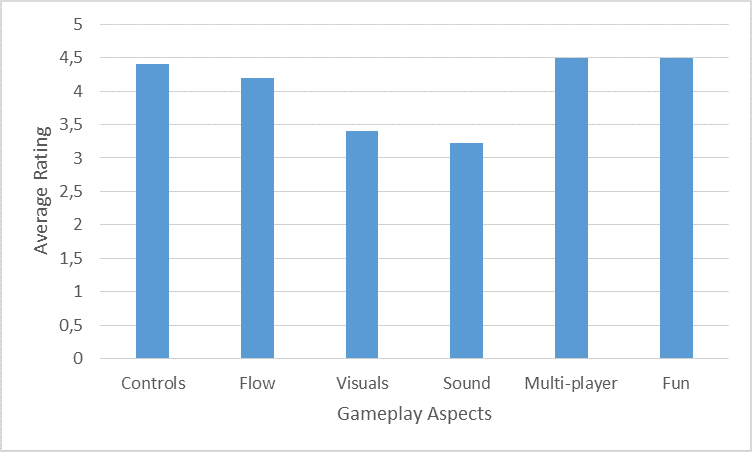
\includegraphics[scale=1]{images/UserTestGraph.png}}
	\caption{Graph showing how users ranked various game-play aspects out of 5}
	\label{fig:userTestGraph}
\end{figure}
\subsubsection{Common user comments}
\begin{description}
	\item [Edge Definition] Edges were not well defined, testers often complained about being unable to differentiate between shadows and gaps.
	\item [Directional Confusion] Confusion as to which direction to go, many users asked for a map or similar functionality be implemented. A significant number of users did mention that colour cues did help with this issue.
	\item [Sound] Ambient sound was not suitable for the game-play, many users said that the sound was too relaxed and that faster, more urgent music would be more suitable
	\item [Controls] Many users commented that the controls were well mapped and intuitive to use
	\item [Multi-player] Most users enjoyed the multi-player aspect of the game saying it made the experience a lot more fun overall
\end{description}
\section{Conclusion}
As specified in our requirements section, we aimed to have a player that can move, jump, slide and grab onto ledges. While we successfully implemented the movement, jumping and sliding, ledge grabbing has yet to be implemented (as can be seen from our validation tests). This is not due to any unforeseen circumstances, rather that the ledge grab functionality was rated to be of a lower priority than the other motions and so insufficient time has been allocated to it before now.
It is important to note that this does not hinder the player's ability to play the game because while ledge grab serves to make the player's motion through the world feel more natural, it does not add to the areas around the world that the player can reach. \\
We managed to successfully implement the player's non-movement-related interaction with the world (re-spawning, smoke grenades, environment interaction and the sniper and drone AI behaviours). \\
While we did successfully add music to our game, it does not transition to a faster pace track during the game. Having background music ensures that the player is not playing in complete silence and adds to the atmosphere of the game world. We initially planned to have the background music transition to faster pace as the game progresses. A more relaxed track would play near the start of the game, but when the player reaches a particular checkpoint in the level, the background music would change to become more intense.
Again the fact that this has not been implemented is mostly down to it being of less importance than the features that more directly affect game-play (such as the AI logic and the player controller). \\
In terms of non-functional requirements, we set out to support a consistently high frame rate, clear visuals, minimal input lag and flow of game-play. We managed to achieve the latter two of these goals and succeeded in the former two to a lesser degree.
While the game runs at a consistent frame rate in most cases, the smoke bomb causes performance issues on some computers. This can be remedied by turning down the render quality settings however, so it is not considered to be a significant problem. \\
The visual style of the game is a success in most cases, it manages to stay clean while not being too bland. However we noticed during user testing that it is necessary to add details to the environment that inform the player of where they should go so as to prevent confusion. This can be achieved by adding decals to the walls around the world, or simply colouring in parts of the environment to draw the player's eye.
While we did manage to add some appropriate colouring to the world, more is needed and decals would greatly improve players' sense of direction while playing but there was no time to add decals before the submission deadline. \\
With regards to project architecture, the Unity engine's built-in object-component model and prefab systems have been successfully used to create easily replaceable, modular units of code which are then pieced together to create the finished product. This functionality, combined with our use of the Model-View-Controller and Layered design patterns have allowed us to create a codebase that can be thought of in reasonably small logical chunks, thereby improving the ability for team members to pick up- and work on a new area of code with comparative ease. Additionally, this modularization allows for easy code re-use since each script fulfills a very specific purpose and can be used to satisfy that purpose in a fairly wide variety of situations and environments within the game.
\\ \\
Overall the project is on-track. We have managed to implement most of the main features so far and already have a playable local-multiplayer running game. As mentioned above there are a few details which remain that would greatly improve the player experience and those will be added in the coming weeks before the final deadline.

\newpage
    \begin{titlepage} \begin{center}
            \textsc{}
            \\[1.5cm] \textsc{} \\\smallskip
            \textsc{} \\\smallskip
            \textsc{} \\\smallskip
            \textsc{} \\\smallskip
            \noindent\rule[0.4mm]{\textwidth}{0.1mm}
            \\[0.4cm] { \huge \bfseries Tempest Trace \\[0.4cm] }
            \noindent\rule[0.4mm]{\textwidth}{0.1mm}
            \\[1cm]
            \textsc{\large{User Manual}}
            \\[14.5cm]
\large{Produced by:\\ Brian Mc George\\ Jacques Heunis\\ Timothy Gwynn}
    \end{center}
\end{titlepage}
\newpage
%Things to add:
%epileptic seizures warning :)
%table of contents
%Getting started (minimum requirements, how to run game, change graphics etc)
%The backstory (use intro dialog?)
%Ref: http://cdn.akamai.steamstatic.com/steam/apps/13580/manuals/manual_english.pdf?t=1307544329
\label{ss:user-manual}
\section*{Getting Started}
\subsection*{Recommended System Requirements}
\begin{description}
    \item \itab{Operating System:}\tab{Windows 7 or greater.}
    \item \itab{Processor:}\tab{Intel i5 2.4Ghz}
    \item \itab{Ram:}\tab{1Gb}
    \item \itab{Video Card:}\tab{DirectX 11 compliant. Nvidia 460 or equivalent.}
    \item \itab{Peripherals:}\tab{Mouse, keyboard or game-pad (Both are required for playing split screen)}
\end{description}
\subsection*{Running the game}
The game is started by running the executable located inside the game's directory.\\
The graphics level and controls can be edited in the window that is displayed when you run the executable.
\section*{Player One Controls}
\begin{description}
    \item \itab{Look:}\tab{Mouse}
    \item \itab{Move forward:}\tab{W}
    \item \itab{Move backward:}\tab{S}
    \item \itab{Move left:}\tab{A}
    \item \itab{Move right:}\tab{D}
    \item \itab{Jump/Climb:}\tab{Spacebar}
    \item \itab{Slide:}\tab{Shift}
    \item \itab{Somkebomb:}\tab{F}
    \item \itab{Object Interaction:}\tab{E}
\end{description}
\section*{Player Two Controls}
\begin{description}
    \item \itab{Look:}\tab{Right Joystick}
    \item \itab{Movement:}\tab{Left Joystick}
    \item \itab{Jump/Climb:}\tab{Left Bumper}
    \item \itab{Slide:}\tab{Right Bumper}
    \item \itab{Somkebomb:}\tab{B Button}
    \item \itab{Object Interaction:}\tab{A Button}
\end{description}
\section*{Background}
Your number is 101010 or three-ten as your fellow slaves know you. You are well known among your fellow’s and many see you as a beacon of hope, the promise of freedom. For you are a free runner and amongst them you are closest to the possibility of freedom. For 6 months you have competed against other slaves to earn the right to take on ``The Mission''.\smallskip\\
Now the final task stands before you, the final race. The next winner will be sent on ``The Mission'' and, should they succeed, they will be granted freedom and a place in society. But it will be no easy challenge, the other runner has passed all the same tests you have, beaten as many opponents and gotten as far as you and is just as determined.\smallskip\\
The course has been readied, there are no camera’s or crowds of people watching as at previous events, only a selected few will see this final test course. The drones have been powered up and their ammo re-filled. If you cannot get past them, you will have no hope of completing ``The Mission''.
\section*{Objective}
Get to the top of the last building before the other player. Move quickly and efficiently while avoiding danger from enemies and falls.
\section*{Enemies}
Flying drones will attempt to chase you down if you get too close to them. Snipers will shoot you if you expose yourself in their field of vision.
\section*{Environment}
Interact with objects such as doors and buttons in your environment by pressing the object interaction button. Buttons will often let you gain a tactical advantage over your opponent.
\section*{Abilities}
Beyond basic movement you can jump, vault, climb and slide over and under objects. If you ever find yourself in trouble with an enemy you can use a smoke bomb to obstruct their vision of you, however you only have 2 of these, so use them wisely! 
\end{document}



